\documentclass[9pt,a4paper]{article}
\usepackage[margin=1.25cm,top=1.55cm,bottom=1.15cm,headsep=0.45cm]{geometry}
\usepackage[T1]{fontenc}
\usepackage[utf8]{inputenc}
\usepackage{lmodern,microtype,graphicx,booktabs,tabularx,array,enumitem,xcolor,hyperref,float,fancyhdr,titlesec,tcolorbox}

\definecolor{OceanTeal}{HTML}{0F766E}
\definecolor{OceanNavy}{HTML}{172B3A}
\definecolor{OceanGold}{HTML}{D97706}
\definecolor{OceanLight}{HTML}{F4F7F9}
\definecolor{OceanGray}{HTML}{536678}
\definecolor{RuleGray}{HTML}{CBD5E1}

\hypersetup{
  colorlinks=true,
  linkcolor=OceanTeal,
  urlcolor=OceanTeal,
  pdftitle={The Rise of Oceanus Folk},
  pdfauthor={Muawia Nasser}
}

\pagestyle{fancy}
\fancyhf{}
\lhead{Visual Analytics 602AA}
\rhead{The Rise of Oceanus Folk}
\cfoot{\thepage}
\renewcommand{\headrulewidth}{0.35pt}
\setlength{\headheight}{13pt}

\titleformat{\section}{\large\bfseries\color{OceanNavy}}{\thesection}{0.55em}{}
\titleformat{\subsection}{\normalsize\bfseries\color{OceanTeal}}{\thesubsection}{0.5em}{}
\titlespacing*{\section}{0pt}{0.55em}{0.28em}
\titlespacing*{\subsection}{0pt}{0.4em}{0.16em}

\setlength{\parindent}{0pt}
\setlength{\parskip}{0.2em}
\setlist[itemize]{leftmargin=1.25em,itemsep=0.06em,topsep=0.1em,parsep=0pt}
\setlist[enumerate]{leftmargin=1.45em,itemsep=0.08em,topsep=0.1em,parsep=0pt}
\renewcommand{\arraystretch}{1.05}
\raggedbottom

\newtcolorbox{simplebox}[1][]{
  colback=white,
  colframe=RuleGray,
  boxrule=0.5pt,
  arc=0.8mm,
  left=2mm,right=2mm,top=1.5mm,bottom=1.5mm,
  #1
}

\newtcolorbox{conceptbox}[1][]{
  colback=OceanLight,
  colframe=OceanTeal,
  boxrule=0.6pt,
  arc=0.8mm,
  left=2.2mm,right=2.2mm,top=1.5mm,bottom=1.5mm,
  #1
}

% A report card uses the real dashboard image on the left and a top-aligned
% explanation on the right. Its height follows the content, so no empty fixed
% image column is created.
\newcommand{\visualcard}[3]{%
  \begin{simplebox}
    \begin{minipage}[t]{0.54\linewidth}
      \vspace{0pt}
      \includegraphics[width=\linewidth]{figures/#2}
    \end{minipage}\hfill
    \begin{minipage}[t]{0.415\linewidth}
      \vspace{0pt}
      \raggedright
      \setlength{\parindent}{0pt}
      {\bfseries\color{OceanNavy}#1}\par
      \vspace{0.8mm}
      \small #3
    \end{minipage}
  \end{simplebox}
  \vspace{1.5mm}
}

\begin{document}

\begin{titlepage}
\thispagestyle{empty}
\begin{center}
{\Large\bfseries\color{OceanNavy}University of Pisa}\par
{\large Department of Data Science and Business Informatics}\par
\vspace{2mm}
\rule{0.92\textwidth}{0.5pt}\par
\vspace{2mm}
{\Huge\bfseries The Rise of Oceanus Folk}\par
{\large\color{OceanTeal}Interactive Visual Analytics of a Music Knowledge Graph}\par
\vspace{2mm}
\rule{0.92\textwidth}{0.5pt}
\end{center}

\vspace{2mm}
\begin{tabularx}{\textwidth}{>{\bfseries\color{OceanNavy}}l X}
Course & Visual Analytics 602AA \\
Professor & Prof. Salvatore Rinzivillo \\
Student & Muawia Nasser \\
Student ID & 725006 \\
Project & VAST Challenge 2025, Mini Challenge 1 \\
Repository & \href{https://github.com/MuawiyaNasser/oceanus-folk-visual-analytics}{github.com/MuawiyaNasser/oceanus-folk-visual-analytics} \\
\end{tabularx}

\vspace{1.5mm}
\begin{conceptbox}
\small\textbf{Project summary.}
The system helps a journalist investigate how Sailor Shift, artists, works, genres, and typed music relationships connect to the rise of Oceanus Folk. Computational summaries prepare the evidence, while linked filtering and selection let the analyst form and verify hypotheses.
\end{conceptbox}

\vspace{2mm}
% The two files are exact horizontal halves of one live dashboard capture.
% offinterlineskip removes the normal baseline gap between consecutive images.
\noindent\makebox[\textwidth][c]{%
  \vbox{\offinterlineskip
    \hbox{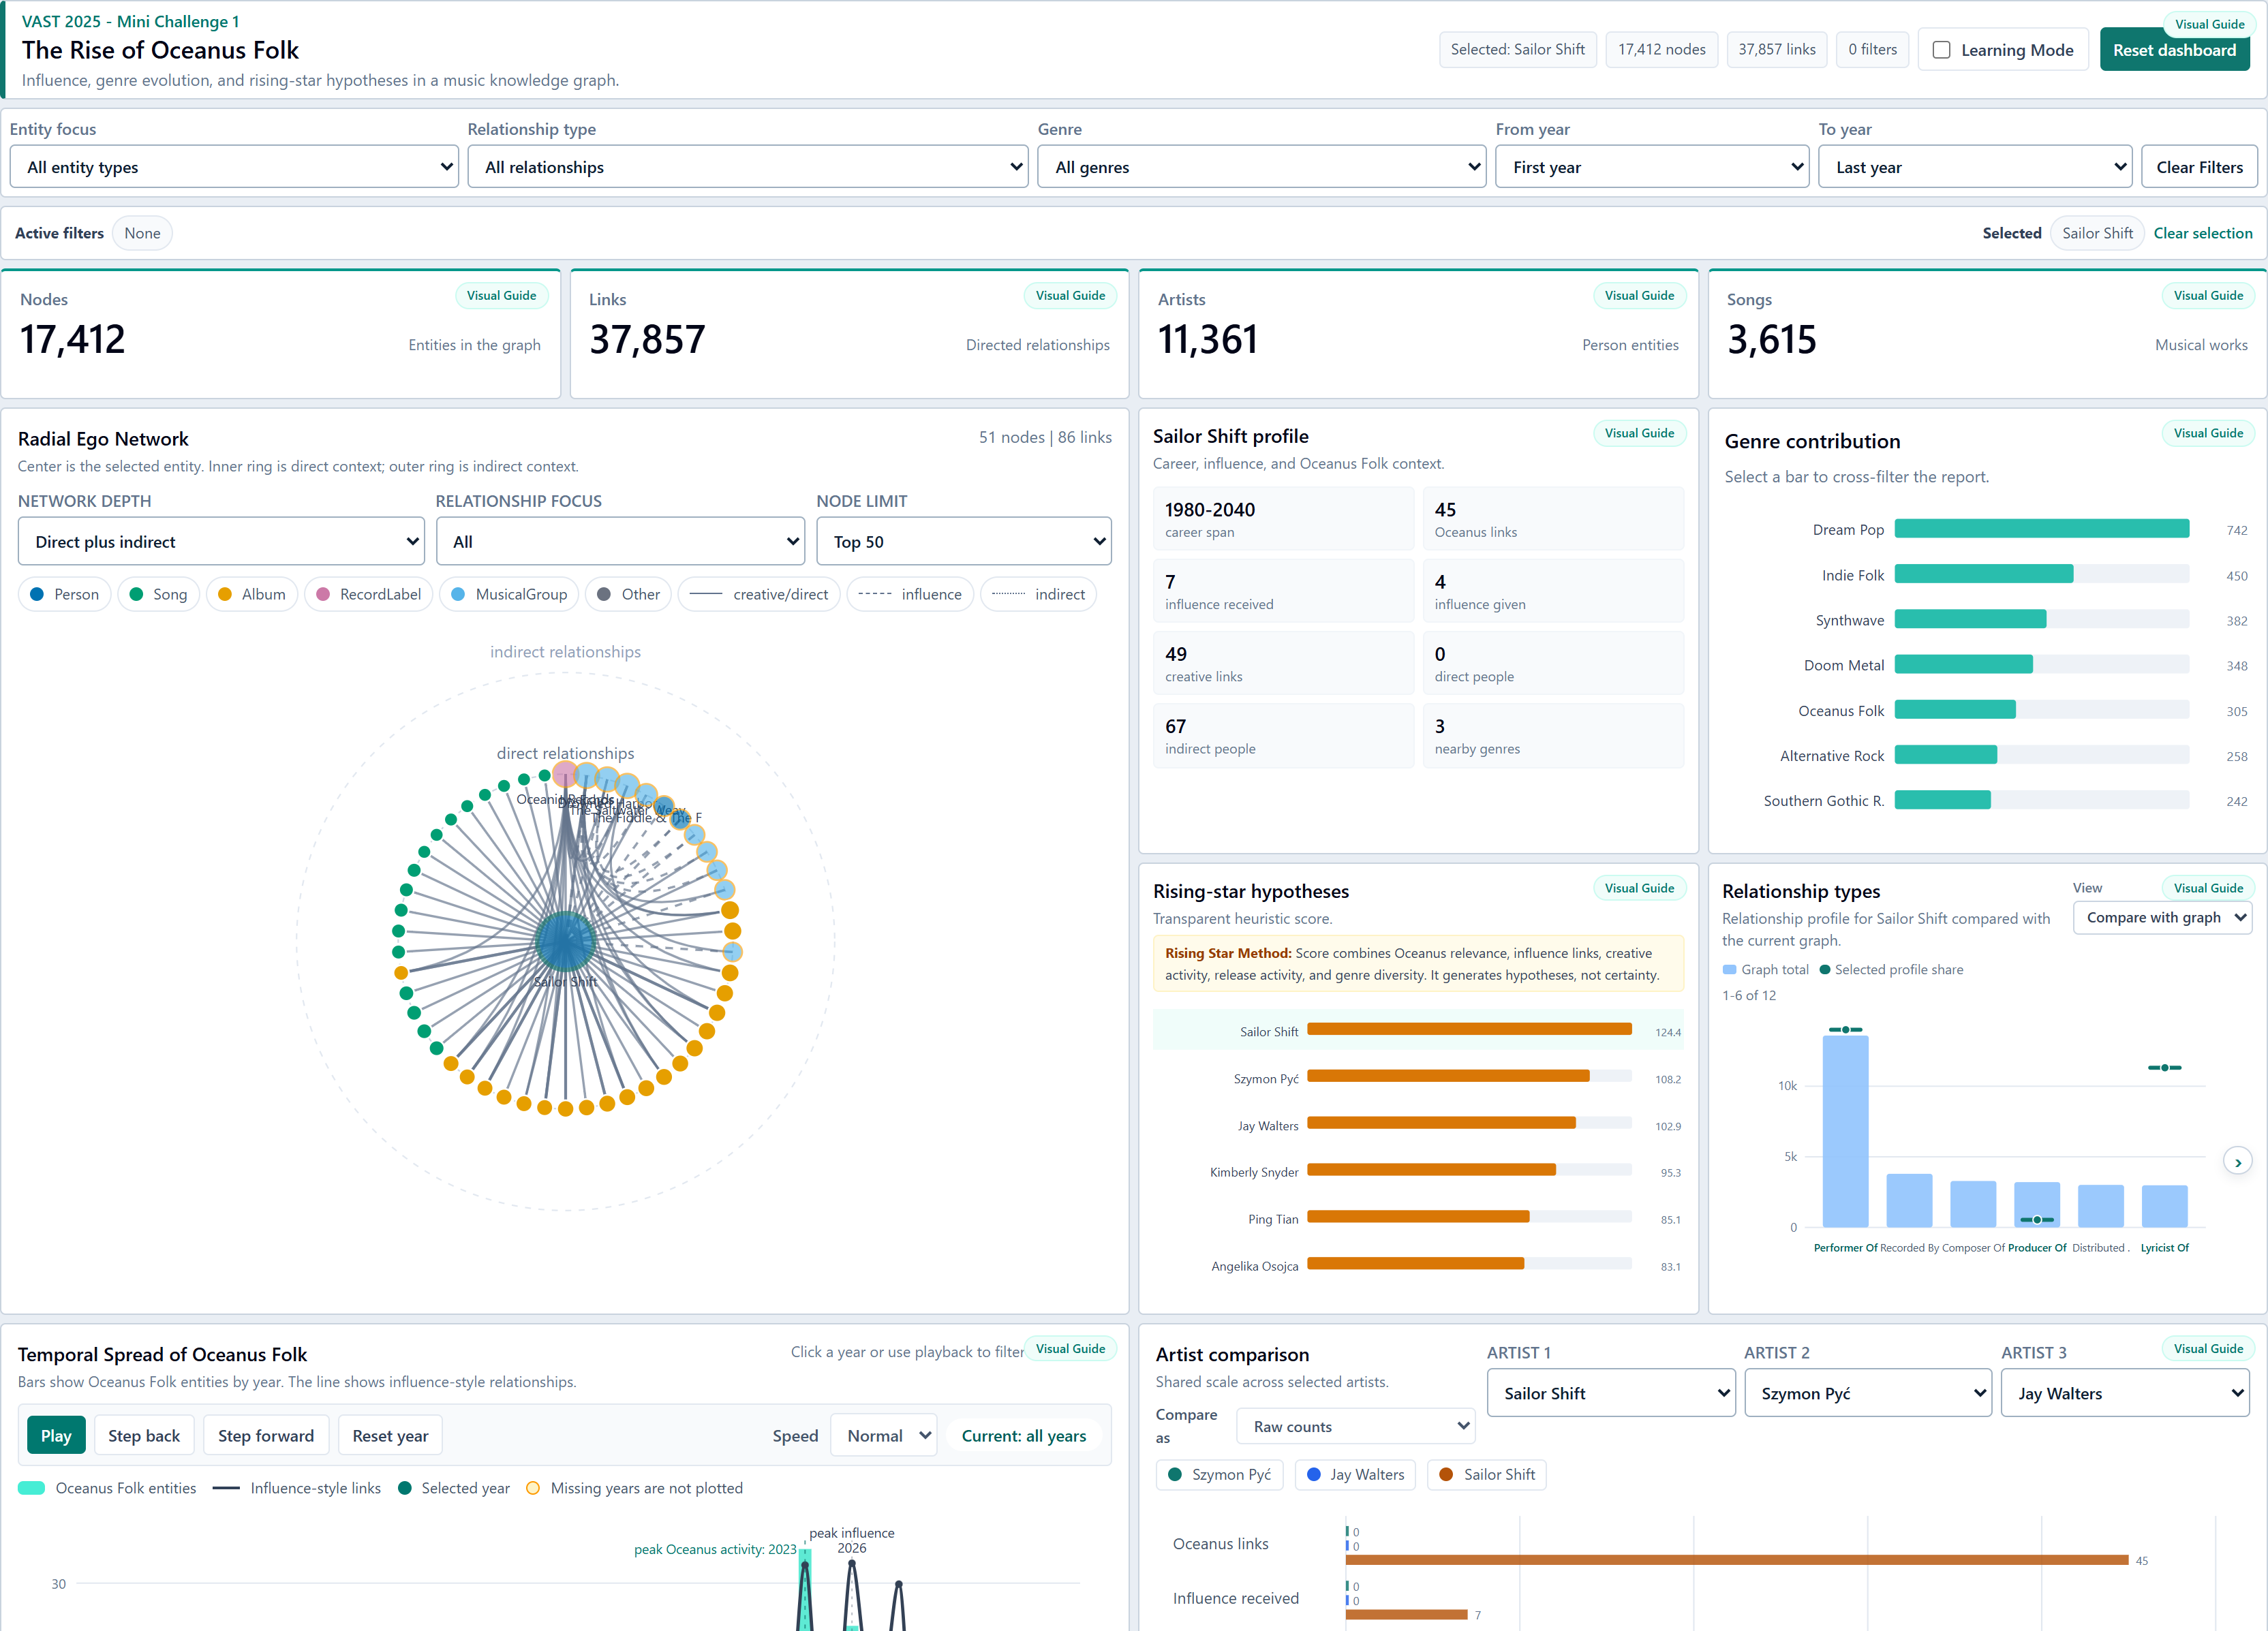
\includegraphics[width=10.5cm]{figures/dashboard_top.png}}
    \hbox{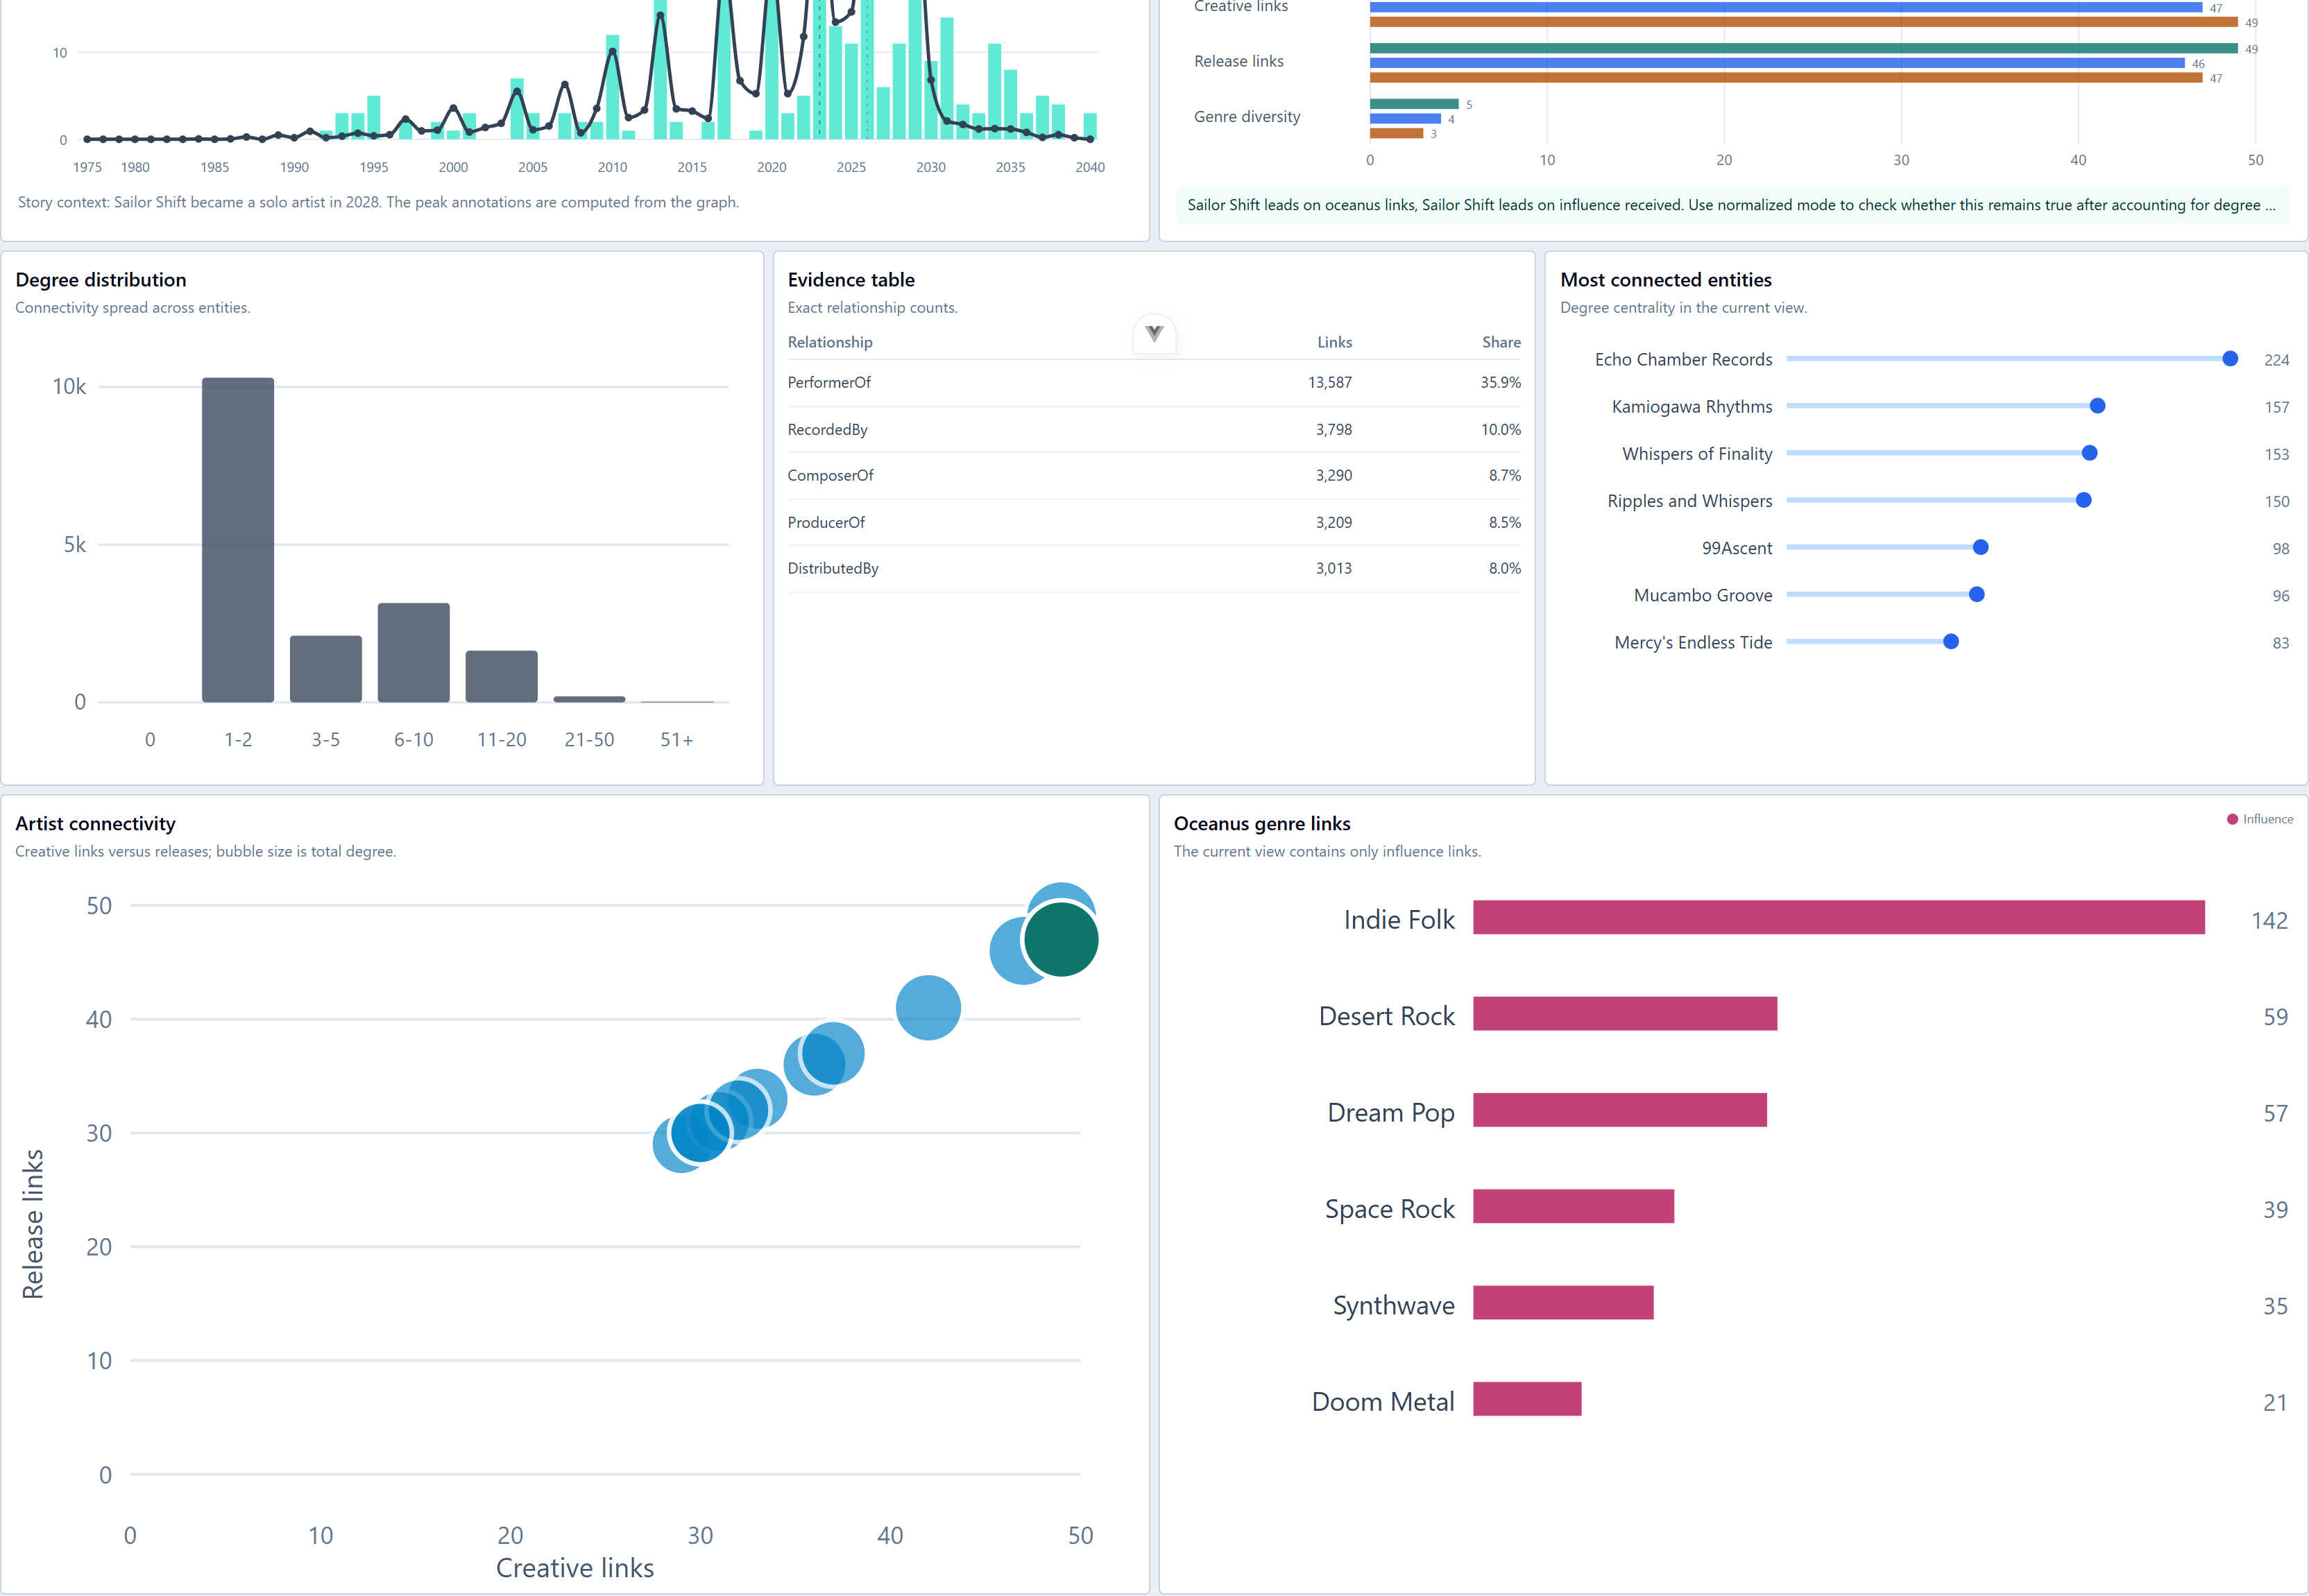
\includegraphics[width=10.5cm]{figures/dashboard_bottom.png}}
  }%
}
\vfill
\begin{center}{\small Academic Year 2025/2026}\end{center}
\end{titlepage}

\section{Introduction and Data}
The project studies the music knowledge graph released for VAST Challenge 2025 Mini Challenge 1. It contains \textbf{17,412 entities} and \textbf{37,857 directed relationships}. Entities include people, songs, albums, record labels, and musical groups. Typed links describe performance, recording, composition, production, distribution, membership, covers, samples, references, and stylistic connections.

A table alone cannot communicate this relational structure, while drawing the complete graph would create an unreadable node--link hairball. The dashboard therefore combines a focused ego network with coordinated statistical views. Each visual answers a specific question and can also refine the analytical state.

\begin{table}[H]\centering\small
\begin{tabularx}{\textwidth}{>{\bfseries}p{2.7cm} >{\raggedright\arraybackslash}X >{\raggedright\arraybackslash}X}
\toprule
Data element & Examples & Dashboard use \\
\midrule
Entities & People, songs, albums, labels, groups & Network nodes, filters, composition, rankings \\
Relationships & PerformerOf, RecordedBy, ComposerOf, ProducerOf & Network edges, evidence, relationship comparison \\
Attributes & Name, entity type, genre, year & Labels, grouping, colour, temporal filtering \\
Derived measures & Degree, creative links, releases, genre diversity & Comparison, distribution, hypotheses \\
\bottomrule
\end{tabularx}
\end{table}

\section{Analytical Goals and Design}
The principal goal is to understand how Oceanus Folk develops through artists, works, genres, and influence. The interface supports questions about Sailor Shift's neighbourhood, temporal growth, dominant relationship types, stylistic bridges, artist profiles, and possible rising stars.

The design follows \emph{overview first, filter and select, details on demand}. KPI cards summarize the visible graph. The radial network receives the largest area because relationships are central to the task. Position and length support quantitative comparison; colour hue separates nominal entity types; line and column marks encode time; and a donut is reserved for the small part-to-whole entity composition. Teal is the dashboard selection accent; blue supports factual comparison; orange signals provisional hypotheses; slate represents neutral structure; rose identifies influence evidence; and the entity palette remains consistent across views. The global controls and direct chart selections update coordinated views, keeping the human analyst in the reasoning loop.

\begin{conceptbox}
\small\textbf{Visual Analytics model.}
The application calculates graph metrics, filtered subsets, rankings, and temporal summaries. The analyst then uses linked visual evidence to compare alternatives, challenge a hypothesis, and return to the complete view through reversible interactions.
\end{conceptbox}

\section{Data Preparation}
The frontend loads the JSON graph, normalizes identifiers and missing values, extracts years, indexes nodes and links, and calculates degree and artist-level measures. Unknown metadata remains explicit instead of being silently invented. The ego network applies a node limit and prioritizes nearby, highly connected entities so that the local graph remains readable.

\clearpage
\section{Dashboard Visuals}

\visualcard{KPI cards}{kpis.png}{
Cards are used because four exact headline values must be scanned faster than they could be read from a chart. They summarize visible nodes, links, artists, and songs and recalculate after global filtering, implementing \emph{overview first}. White surfaces and dark text maximize legibility, while the thin teal rule links the cards to the dashboard's analytical accent without making the numbers compete with decorative colour.
}

\visualcard{Radial ego network}{network.png}{
A radial ego network is used because the task concerns relationships around one focus entity, and rings communicate direct versus indirect distance more clearly than a free force layout. The centre is selected; \textbf{Network Depth}, \textbf{Relationship Focus}, and \textbf{Node Limit} control scope and clutter. A consistent colour-blind-aware categorical palette maps people to blue, songs to green, albums to amber, labels to pink, groups to sky blue, and other types to gray. Teal outlines emphasize selection, amber outlines flag unknown genre metadata, node size reflects degree, and restrained gray edge styles distinguish direct, influence, and indirect relations. Hover and click provide details and refocusing.
}

\visualcard{Genre contribution}{genre_contribution.png}{
A sorted horizontal bar chart is used because this is a categorical ranking with long genre names; aligned length on a common baseline supports accurate comparison. Teal bars connect the view to genre selection and Oceanus-related exploration, while pale gray tracks preserve the full comparison range and make filtering changes visible. The darker teal active bar is consistent with the dashboard selection colour. Clicking a genre cross-filters linked views, clicking it again clears it, and the ranking updates after other filters.
}

\clearpage
\section{Dashboard Visuals Continued}

\visualcard{Entity composition}{entity_composition.png}{
A donut is appropriate because a small number of entity categories partition one meaningful whole. The centre reports the visible total, while slice angles and percentages communicate composition. Colours deliberately match the network: people are blue, songs green, labels pink, albums amber, and groups sky blue. This cross-view consistency reduces relearning and uses hue only for nominal categories. Filtering updates the centre value, slices, and legend to show which entity type dominates the current context.
}

\visualcard{Rising-star hypotheses}{rising_stars.png}{
A sorted horizontal bar chart is chosen because candidates must be ranked on one transparent heuristic score, and aligned lengths are easier to compare than areas or angles. Orange is used deliberately as a cautionary, provisional colour: the score generates hypotheses and is not established truth. A pale teal row identifies the currently selected candidate without changing the score encoding. Selecting a candidate updates the network and artist comparison so the ranking starts an investigation rather than ending it.
}

\visualcard{Relationship types}{relationship_types.png}{
A column chart is suitable because the relationship names are short and the goal is comparison of discrete counts from a shared zero baseline. Column height encodes the frequency of PerformerOf, RecordedBy, ComposerOf, ProducerOf, DistributedBy, and LyricistOf. Calm blue represents factual structural evidence rather than selection or warning, while teal is reserved for an active category. The chart updates after filtering and reveals which link type dominates the current context.
}

\clearpage
\section{Dashboard Visuals Continued}

\visualcard{Oceanus Folk timeline}{timeline.png}{
A combined column-and-line chart is used because it compares two temporal signals without hiding their different mark types: aqua columns show yearly Oceanus Folk activity and a dark navy line shows influence-style relationships. Aqua connects activity to the dashboard's Oceanus accent; navy provides strong contrast for the second measure; dark teal identifies the selected year; and amber marks missing-year uncertainty. Time runs left to right and peak annotations guide interpretation. Click, playback, step controls, speed, and reset coordinate the selected year with the other views.
}

\visualcard{Artist comparison}{artist_comparison.png}{
Grouped horizontal bars are used because three artists must be compared repeatedly across the same measures on shared axes. Teal, blue, and burnt orange give each artist a stable, distinguishable identity across every metric without implying good or bad performance; neutral gridlines keep attention on bar length. Measures include Oceanus links, influence received and given, creative links, release links, and genre diversity. Raw counts show absolute evidence, while normalization by degree or releases supports fairer comparison. Selectors replace artists and chart selection can change the active focus.
}

\visualcard{Degree distribution}{degree_distribution.png}{
A histogram is the appropriate choice because degree is quantitative and the question concerns its distribution, not a ranking of named entities. Bins reduce thousands of individual degrees into readable intervals and reveal many low-degree entities versus a few hubs. Slate is intentionally neutral because this chart describes background graph structure rather than an active category; its subdued tone prevents the large first bin from dominating the dashboard. The histogram recalculates after filtering.
}

\clearpage
\section{Dashboard Visuals Continued}

\visualcard{Evidence table}{evidence_table.png}{
A compact table is used instead of a chart because the task here is verification of exact relationship counts and shares. It complements the pattern-oriented visuals and remains intentionally short. Colour is minimized: dark text carries the values, light gray rules organize rows, and the white surface avoids assigning unsupported semantic meaning to categories. This restrained treatment keeps exact evidence readable without competing with interactive selections.
}

\visualcard{Most connected entities}{connected_entities.png}{
A lollipop chart is chosen for a compact degree ranking: aligned dot positions preserve bar-chart accuracy while using less ink. Entities are sorted so the strongest hubs appear first. Blue dots communicate factual centrality consistently with other structural comparisons, pale blue stems provide scale context, and teal marks the selected entity. Clicking a dot moves from the ranking to that entity's local network evidence.
}

\visualcard{Artist connectivity}{artist_connectivity.png}{
A bubble scatterplot is used because two quantitative variables must be compared simultaneously: creative links on the horizontal axis and release links on the vertical axis. Bubble area adds total degree as a third measure. Context artists use sky blue, a calm comparison colour distinct from the rose influence and orange hypothesis encodings; the selected artist turns teal, and white outlines separate overlaps. Clicking a bubble selects the artist, revealing profiles that a single ranking would hide.
}

\clearpage
\section{Dashboard Visuals Continued}

\visualcard{Oceanus genre links}{oceanus_genre_links.png}{
A horizontal bar chart ranks external genres connected to Oceanus Folk, which gives long labels room and uses aligned length for accurate comparison. The aggregation assigns every link to exactly one class: Influence, Creative, or Other. The current data contains only Influence links for the displayed genres, so zero-value categories are hidden and the chart states this limitation. Rose is reserved for influence evidence, distinguishing it from teal selection and orange creative evidence. Clicking a genre applies the linked genre filter.
}

\section{Interaction Model}
All views share one understandable analytical state: selected entity, entity type, relationship type, genre, and year range. Network depth and node limit control only the local graph presentation. A chart selection is highlighted, related views update, a repeated click clears the selection where applicable, and \textbf{Reset filters} restores Sailor Shift and the full dataset.

\begin{table}[H]\centering\small
\begin{tabularx}{\textwidth}{>{\bfseries}p{2.7cm} >{\raggedright\arraybackslash}X >{\raggedright\arraybackslash}X}
\toprule
Action & Coordinated response & Analytical purpose \\
\midrule
Click a node or ranked entity & Network recentres; details and comparison update & Move from overview to local evidence \\
Click a genre or relationship & Linked charts and graph subset update & Isolate one categorical explanation \\
Click or play a year & Applicable views recalculate for that period & Examine temporal development \\
Change artist selectors or mode & Shared measures are redrawn & Compare absolute and normalized profiles \\
Reset filters & Full graph state and Sailor Shift return & Keep exploration reversible \\
\bottomrule
\end{tabularx}
\end{table}

\section{State of the Art and Original Contribution}
The dashboard follows coordinated-view practices common to Tableau, Power BI, and other visual analytics systems: compact controls, KPI feedback, linked charts, highlighting, and details on demand. Knowledge-graph tools commonly use node--link diagrams, matrices, or search-based exploration. The original D3 contribution is the radial ego network, which replaces an unconstrained force layout with explicit distance rings, relationship controls, degree-based sizing, and a readable subset rule.

\clearpage
\section{Analytical Use Case}
A music journalist begins with Sailor Shift and reads the KPI overview. The analyst changes Relationship Focus to influence, examines direct and indirect neighbours, and selects a peak period in the timeline. The genre views reveal external stylistic connections, while the rising-star hypotheses suggest candidates for closer inspection. A candidate is selected, compared with Sailor Shift and another artist in raw and normalized modes, and then checked through the local network, centrality ranking, genre-link composition, and exact evidence table. The result is a traceable hypothesis supported by several coordinated views rather than one automatic score.

\section{Implementation}
The project uses Vue, JavaScript, CSS, SVG, and D3. The code flow remains deliberately simple: load and normalize the graph, hold the shared dashboard state, apply filters, compute derived metrics, and render reusable visual components. D3 scales map values to position, length, radius, and colour. Vue propagates state changes so that one interaction updates all relevant components.

\section{Limitations}
Some entities lack reliable genre or year metadata. Unknown values remain visible or are excluded only where explicitly stated, so missing data can affect rankings and temporal interpretation. Degree measures connectivity, not artistic quality. Influence-style links reflect the available graph relationships and do not prove causality. The rising-star score is therefore an explainable hypothesis generator, not a forecast with statistical certainty. The dashboard uses focused subsets to reduce cognitive overload, which means that the radial network is intentionally not a complete graph view.

\section{Conclusion}
The project turns a large music knowledge graph into a compact analytical workspace. Computational summaries expose candidate patterns, while linked interaction lets the user test them across relationships, time, genres, and artist profiles. Appropriate visual variables, consistent scales, reversible filtering, and details on demand reduce cognitive load and support human-in-the-loop reasoning.

\section*{Acknowledgement of AI-Assisted Development}
OpenAI Codex was used as a development assistant for implementation, debugging, refactoring, visual quality checks, and report preparation. The analytical direction, project decisions, interpretation, and final responsibility remain with the author.

\begin{conceptbox}
\small\textbf{Final point.}
This is a Visual Analytics system rather than a static collection of charts: computation prepares evidence, coordinated visualization exposes patterns, and interaction lets the analyst refine and verify an interpretation.
\end{conceptbox}

\end{document}
